\begin{figure}
	\definecolor{myorange}{RGB}{252,141,98}
	\definecolor{mygreen}{RGB}{102,194,165}
	\definecolor{myblue}{RGB}{141,160,203}
\centering
\begin{minipage}{0.32\textwidth}
\centering
\resizebox{\linewidth}{!}{
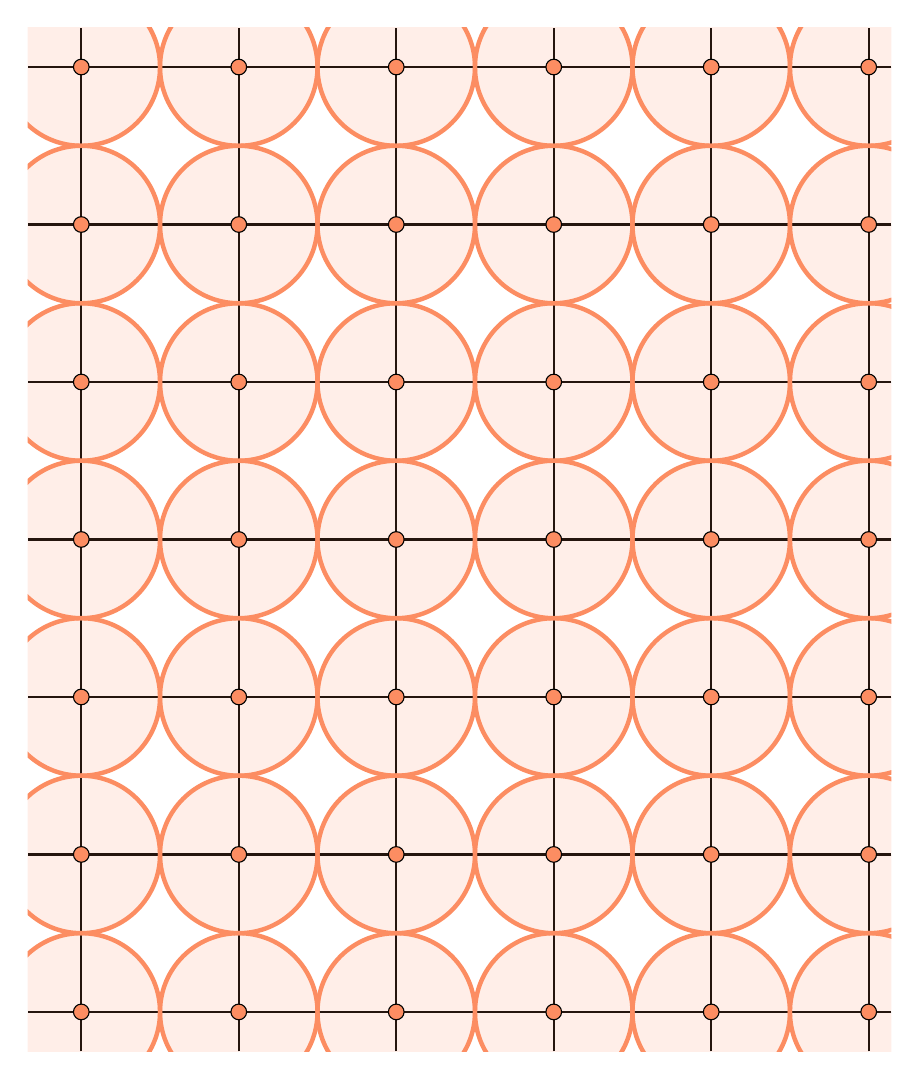
\begin{tikzpicture}[rotate=90]
  \clip (-0.5,{-sqrt(3)/6}) rectangle (12.5,{18.5/3*sqrt(3)});

\foreach \j in {0,...,6} {
  \def\y{{\j*2}}
  \draw [thick] (-0.5,\y) -- (12.5,\y);
}
\foreach \i in {0,...,6} {
  \def\x{{\i*2}}
  \draw [thick] (\x,{-sqrt(3)/3*0.5}) -- (\x,{18.5/3*sqrt(3)});
}

\foreach \i in {0,...,6} {
  \foreach \j in {0,...,6} {
    %\ifnum \numexpr(mod(\i+\j,2))=0
    \def\x{{2*\i}}
    \def\y{{2*\j}}
    \filldraw[color=myorange, fill=myorange, fill opacity=0.15, ultra thick](\x,\y) circle (1);
    \node[circle,fill=myorange,draw=black,inner sep=2pt] () at (\x,\y) {};
  }
}
\end{tikzpicture}
}
\end{minipage}
\begin{minipage}{0.32\textwidth}
\centering
\resizebox{\linewidth}{!}{
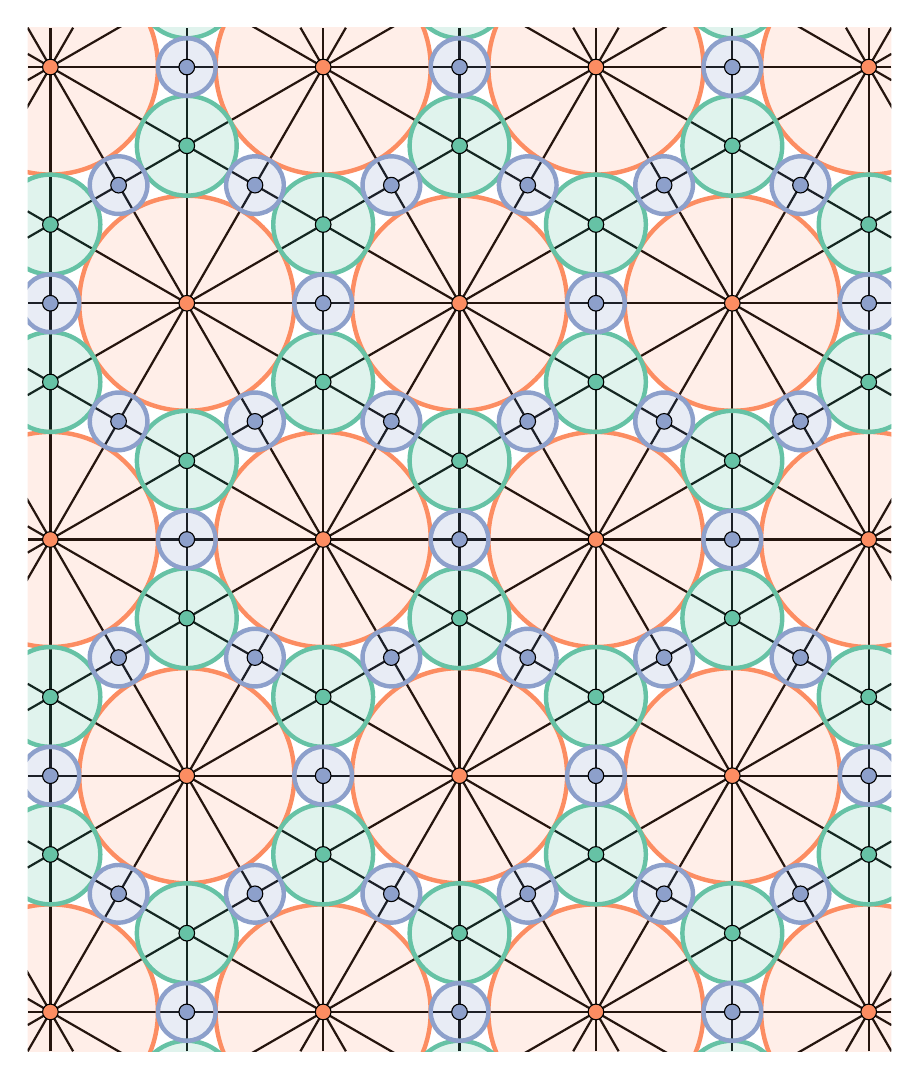
\begin{tikzpicture}[rotate=90]
  \clip (-0.5,{-sqrt(3)/6}) rectangle (12.5,{18.5/3*sqrt(3)});

% edges 
\foreach \j in {0,...,6} {
  \def\y{{\j*sqrt(3)}}
  \draw [thick] (-0.5,\y) -- (12.5,\y);
}
\foreach \i in {0,...,4} {
  \def\x{{\i*3}}
  \draw [thick] (\x,{-sqrt(3)/3*0.5}) -- (\x,{18.5/3*sqrt(3)});
}

\foreach \i in {0,...,5} {
  \def\x{{(6*\i-12-0.5)*sqrt(3)/3}}
  \def\y{{(6*\i+0.5)*sqrt(3)/3}}
  \draw [thick] (-0.5,\x) -- (12.5,\y);
  \draw [thick] (12.5,\x) -- (-0.5,\y);
}

\foreach \i in {0,...,9} {
  \def\x{{2*\i-37/6}}
  \def\y{{2*\i+1/6}}
  \draw [thick] (\x,{37/6*sqrt(3)}) -- (\y,{-1/6*sqrt(3)});
  \draw [thick] (\y,{37/6*sqrt(3)}) -- (\x,{-1/6*sqrt(3)});
}

% myorange
\foreach \i in {0,...,4} {
  \foreach \j in {0,...,6} {
    %\ifnum \numexpr(mod(\i+\j,2))=0
    \def\x{{3*\i}}
    \def\y{{sqrt(3)*\j}}
    \pgfmathparse{{int(mod(\i+\j,2))}}
    \ifnum \pgfmathresult=0
      {
        \filldraw[color=myorange, fill=myorange, fill opacity=0.15, ultra thick](\x,\y) circle ({(1+sqrt(3))/2});
        \node[circle,fill=myorange,draw=black,inner sep=2pt] () at (\x,\y) {};
      }
    \fi
  }
}
% mygreen
\foreach \i in {-1,...,4} {
  \foreach \j in {0,...,6} {
    %\ifnum \numexpr(mod(\i+\j,2))=0
    \def\xa{{3*\i+1}}
    \def\xb{{3*\i+2}}
    \def\y{{sqrt(3)*\j}}
    \pgfmathparse{{int(mod(\i+\j,2))}}
    \ifnum \pgfmathresult=0
      {\filldraw[color=mygreen, fill=mygreen, fill opacity=0.2, ultra thick](\xb,\y) circle ({(3-sqrt(3))/2});
      \node[circle,fill=mygreen,draw=black,inner sep=2pt] () at (\xb,\y) {};}
    \else
      {\filldraw[color=mygreen, fill=mygreen, fill opacity=0.2, ultra thick](\xa,\y) circle ({(3-sqrt(3))/2});
      \node[circle,fill=mygreen,draw=black,inner sep=2pt] () at (\xa,\y) {};}
    \fi
  }
}
% myblue
\foreach \i in {0,...,4} {
  \foreach \j in {0,...,6} {
    %\ifnum \numexpr(mod(\i+\j,2))=0
    \def\x{{3*\i}}
    \def\y{{sqrt(3)*\j}}
    \pgfmathparse{{int(mod(\i+\j,2))}}
    \ifnum \pgfmathresult=1
      {\filldraw[color=myblue, fill=myblue, fill opacity=0.2, ultra thick](\x,\y) circle ({(sqrt(3)-1)/2});
      \node[circle,fill=myblue,draw=black,inner sep=2pt] () at (\x,\y) {};}
    \fi
  }
}
\foreach \i in {0,...,3} {
  \foreach \j in {0,...,5} {
    %\ifnum \numexpr(mod(\i+\j,2))=0
    \def\x{{3*\i+1.5}}
    \def\y{{sqrt(3)*\j+sqrt(3)/2}}
    \filldraw[color=myblue, fill=myblue, fill opacity=0.2, ultra thick](\x,\y) circle ({(sqrt(3)-1)/2});
    \node[circle,fill=myblue,draw=black,inner sep=2pt] () at (\x,\y) {};
  }
}
\end{tikzpicture}
}
\end{minipage}
\begin{minipage}{0.32\textwidth}
\centering
\resizebox{\linewidth}{!}{
\begin{tikzpicture}

\filldraw[color=myorange, fill=myorange, fill opacity=0.15, ultra thick](0:0) circle (1);
\node[circle,fill=myorange,draw=black,inner sep=2pt] () at (0:0) {};

\foreach \i in {0,...,2} {
    \def\t{360/3*\i+360/6}
    \def\r{2}
    \def\s{1}
    \filldraw[color=myblue, fill=myblue, fill opacity=0.2, ultra thick](\t:\r) circle (\s);
    \node[circle,fill=myblue,draw=black,inner sep=2pt] () at (\t:\r) {};
    \begin{scope}[on background layer]
      \draw[thick] (\t:\r) -- (0,0);
    \end{scope}
}

\foreach \i in {0,...,5} {
    \def\t{360/6*\i+360/12}
    \def\r{{sqrt(3)*2}}
    \def\s{1}
    \filldraw[color=mygreen, fill=mygreen, =0.5, fill opacity=0.2, ultra thick](\t:\r) circle (\s);
    \node[circle,fill=mygreen,draw=black,inner sep=2pt] () at (\t:\r) {};
    \begin{scope}[on background layer]
      \def\tt{{360/3*int(\i/2)+360/6}}
      \def\rr{{2}}
      \draw[thick] (\t:\r) -- (\tt:\rr);
    \end{scope}
}

\foreach \i in {0,...,11} {
    \def\t{360/12*\i+360/24}
    \def\r{5.13384}
    \def\s{1}
    \filldraw[color=myorange, fill=myorange, fill opacity=0.15, ultra thick](\t:\r) circle (\s);
    \node[circle,fill=myorange,draw=black,inner sep=2pt] () at (\t:\r) {};
    \begin{scope}[on background layer]
      \def\tt{{360/6*int(\i/2)+360/12}}
      \def\rr{{sqrt(3)*2}}
      \draw[thick] (\t:\r) -- (\tt:\rr);
    \end{scope}
}

\foreach \i in {0,...,23} {
    \def\t{360/24*\i+360/48}
    \def\r{6.63}
    \def\s{0.6667}
    \filldraw[color=myblue, fill=myblue, fill opacity=0.2, ultra thick](\t:\r) circle (\s);
    \node[circle,fill=myblue,draw=black,inner sep=2pt] () at (\t:\r) {};
    \begin{scope}[on background layer]
      \def\tt{{360/12*int(\i/2)+360/24}}
      \def\rr{5.13384}
      \draw[thick] (\t:\r) -- (\tt:\rr);
    \end{scope}
}

\foreach \i in {0,...,47} {
    \def\t{360/48*\i+360/96}
    \def\r{7.6}
    \def\s{0.4}
    \filldraw[color=mygreen, fill=mygreen, fill opacity=0.2, ultra thick](\t:\r) circle (\s);
    \node[circle,fill=mygreen,draw=black,inner sep=2pt] () at (\t:\r) {};
    \begin{scope}[on background layer]
      \def\tt{{360/24*int(\i/2)+360/48}}
      \def\rr{6.63}
      \draw[thick] (\t:\r) -- (\tt:\rr);
    \end{scope}
}

\foreach \i in {0,...,95} {
    \def\t{360/96*\i+360/192}
    \def\r{8.2}
    \def\s{0.24}
    \filldraw[color=myorange, fill=myorange, fill opacity=0.15, ultra thick](\t:\r) circle (\s);
    \node[circle,fill=myorange,draw=black,inner sep=2pt] () at (\t:\r) {};
    \begin{scope}[on background layer]
      \def\tt{{360/48*int(\i/2)+360/96}}
      \def\rr{7.6}
      \draw[thick] (\t:\r) -- (\tt:\rr);
    \end{scope}
}

\end{tikzpicture}
}
\end{minipage}
\par
\begin{minipage}{0.32\textwidth}
\centering
\caption*{(a)}
\end{minipage}
\begin{minipage}{0.32\textwidth}
\centering
\caption*{(b)}
\end{minipage}
\begin{minipage}{0.32\textwidth}
\centering
\caption*{(c)}
\end{minipage}

\caption{Circle packings of some lattices. (a): $\mathbb{Z}^2$ grid, $R=1$. (b): Kisrhombille tiling, $R=2-\sqrt{3}$. (c): degree-$3$ Bethe lattice, $R=0$.}
\label{fig:packing}
\end{figure}
